 
% Copyright 2004 by Till Tantau <tantau@users.sourceforge.net>.
%
% In principle, this file can be redistributed and/or modified under
% the terms of the GNU Public License, version 2.
%
% However, this file is supposed to be a template to be modified
% for your own needs. For this reason, if you use this file as a
% template and not specifically distribute it as part of a another
% package/program, I grant the extra permission to freely copy and
% modify this file as you see fit and even to delete this copyright
% notice. 
\AtBeginDocument{\renewcommand{\bibname}{References}}

\documentclass{beamer}
%\usepackage[table]{xcolor}
\usepackage[absolute,overlay,showboxes]{textpos}
\usepackage{caption}
\usepackage{xcolor,colortbl}
\usepackage{amsmath}

\usepackage{amsthm}
\usepackage{amssymb}
\usepackage{amsmath}
\usepackage{graphicx}
\usepackage{subfigure}
\usepackage{float}
% \usepackage{epstopdf}
\usepackage{tikz}
\usetikzlibrary{intersections}
\usetikzlibrary{through}
\usetikzlibrary{angles}
\usetikzlibrary{calc}
\usetikzlibrary{quotes}
%\usepackage{hyperref}



% 
% \usepackage[bottom]{footmisc}
% 
% \usepackage[figure,table]{hypcap}
\usepackage{verbatim}

%\AtBeginDocument{\renewcommand{\bibname}{References}}

% There are many different themes available for Beamer. A comprehensive
% list with examples is given here:
% http://deic.uab.es/~iblanes/beamer_gallery/index_by_theme.html
% You can uncomment the themes below if you would like to use a different
% one:
%\usetheme{AnnArbor}
%\usetheme{Antibes}
%\usetheme{Bergen}
%\usetheme{Berkeley}
%\usetheme{Berlin}
%\usetheme{Boadilla}
%\usetheme{boxes}
%\usetheme{CambridgeUS}
%\usetheme{Copenhagen}
%\usetheme{Darmstadt}
\usetheme{default}
%\usetheme{Frankfurt}
%\usetheme{Goettingen}
%\usetheme{Hannover}
%\usetheme{Ilmenau}
%\usetheme{JuanLesPins}
%\usetheme{Luebeck}
%\usetheme{Madrid}
%\usetheme{Malmoe}
%\usetheme{Marburg}
%\usetheme{Montpellier}
%\usetheme{PaloAlto}
%\usetheme{Pittsburgh}
%\usetheme{Rochester}
%\usetheme{Singapore}
%\usetheme{Szeged}
%\usetheme{Warsaw}

\title{Sojourn Time of Moving Relays in Dual-Hop Cooperative Communication}

% A subtitle is optional and this may be deleted
%\subtitle{Dual Degree Phase 1 Presentation}

\author{Prudhvi Porandla \\ 110070039\\}

%\vspace{2mm}
%Guide: Prof. S. N. Merchant \\
%\vspace{2mm}
%Dual Degree Phase 1 Presentation}

% - Give the names in the same order as the appear in the paper.
% - Use the \inst{?} command only if the authors have different
%   affiliation.

% - Use the \inst command only if there are several affiliations.
% - Keep it simple, no one is interested in your street address.

\date{June 20, 2016}
% - Either use conference name or its abbreviation.
% - Not really informative to the audience, more for people (including
%   yourself) who are reading the slides online

%%%%%\subject{Theoretical Computer Science}
% This is only inserted into the PDF information catalog. Can be left
% out. 

% If you have a file called "university-logo-filename.xxx", where xxx
% is a graphic format that can be processed by latex or pdflatex,
% resp., then you can add a logo as follows:

% \pgfdeclareimage[height=0.5cm]{university-logo}{university-logo-filename}
% \logo{\pgfuseimage{university-logo}}

% Delete this, if you do not want the table of contents to pop up at
% the beginning of each subsection:


% Let's get started
\begin{document}

\begin{frame}
  \titlepage
\end{frame}

\begin{frame}{Overview}
  \begin{itemize}
  \item Introduction
  \vspace{3mm}
  \item Problem Formulation
  \vspace{3mm}
  \item Simulations
  \vspace{3mm}
  \item Further Work
  \vspace{3mm}
  \end{itemize}
  % You might wish to add the option [pausesections]
\end{frame}

%----------------------------------------------------------------------------------------------------------------------------------------%

% Section and subsections will appear in the presentation overview
% and table of contents.

\section{Introduction}
\frame{\sectionpage}

\begin{frame}{Downlink Cooperation policy}
  A cooperation policy for downlink can be defined along the same lines as we did in uplink 
case. Let $P_b$ be the transmission power used by the base station and $P_r$ be relay power. A simple distance based policy would be
\begin{equation*}
	\{P_b r_1^{-\alpha} > P_b R_0^{-\alpha}, P_rr_2^{-\alpha} > P_bR_0^{-\alpha}\} 
\end{equation*}

\begin{figure}[h]
	\centering \vspace{-0.1in}

	\begin{tikzpicture}[scale=0.05]
		\coordinate [label=left:{\small $BS$}] (A) at (0,0);
		\fill [red,opacity=.5] (A) circle (50pt);

		\coordinate [label=right:{\small $U$}] (B) at (150,0);
		\fill [green,opacity=.5] (B) circle (50pt);

		\coordinate [label=above:{\small $Relay$}] (C) at (125,50);
		\fill [blue,opacity=.5] (C) circle (50pt);

		\draw (A) -- node[below=2pt] {\small $R_0$} (B) -- node[right=2pt] {\small $r_2$} (C)
												-- node[above=2pt] {\small $r_1$} cycle;

	\end{tikzpicture}

	\vspace{-10pt} \caption[Distances for Downlink Cooperation]{\small Distances for Downlink Cooperation}
	\label{fig:dwnlink}
\end{figure}

\end{frame}

\begin{frame}

It can be rewritten as $\{ r_1 < R_0, r_2 < R_2 \}$ where $R_2 = cR_0, c = \big(\frac{P_r}{P_b}\big)^{\frac{1}{\alpha}} $ and $r_1, r_2$ are as defined in the figure \ref{fig:dwnlink}.  
The two conditions in the policy ensure that both BS-relay and relay-user links are stronger than BS-user link. The policy dictates that the idle user should be located in the shaded part of figure \ref{fig:region} to be considered for relaying.

\begin{figure}[h]
	\centering \vspace{0.1in}

	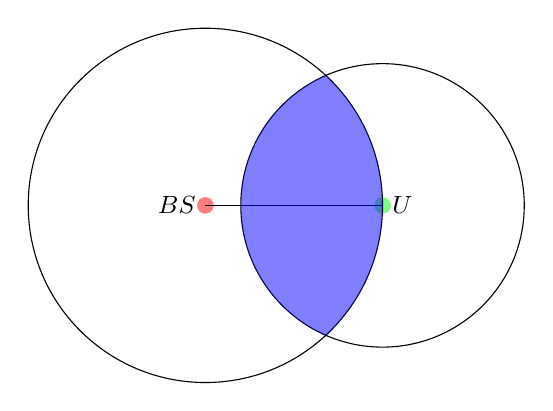
\begin{tikzpicture}[scale=0.015]
		\coordinate [label=left:{\small $BS$}] (A) at (0,0);
		\coordinate [label=right:{\small $U$}] (B) at (150,0);
		\fill [red,opacity=.5] (A) circle (200pt);
		\fill [green,opacity=.5] (B) circle (200pt);

		\draw (A) -- (B);
		\node (D) [name path=D,draw,circle through=(B)] at (A) {};
		%	\node (E) [name path=E,draw,circle(60)] at (B);
		% Name the coordinates, but do not draw anything:
		\draw (B) circle(120);
		\begin{scope}
			\clip (0,0) circle(150);
			\fill[blue,opacity=.5] (150,0) circle (120);
		\end{scope}
		%	\path [name intersections={of=D and E}];
	\end{tikzpicture}

	\vspace{-5pt} \caption[Feasible region]{\small Feasible region}
	\label{fig:region}
\end{figure}

\end{frame}
%%%%\section{Second Main Section}

\begin{frame}{Mobile Relays} {Definitions}
We define mobility more formally and introduce the model proposed in \cite{lin}. The $n$th transition of a node can be denoted by the parameters set $(\mathbf{X}_{n-1},\mathbf{X}_n, V_n, S_n) $. $X_{n-1}$ denotes the starting waypoint and $X_N$ denotes the destination. In addition to the transition time which can be obtained from velocity $V_n$, pause time or thinking time ($S_n$) at destination can also be included in the description of mobility. 
Different mobility models can be distinguished by the distribution of transition length($L_n = \|\mathbf{X}_{n-1} - \mathbf{X}_n \|$) and the distribution of angle made by the vector
$\mathbf{X}_n - \mathbf{X}_{n-1}$ w.r.t x-axis. 
\end{frame}

\begin{frame}{Rayleigh RWP}
In Rayleigh RWP, the angle is chosen uniformly from $[0,2\pi]$ and the transition length is rayleigh distributed with parameter $\lambda$. 
\begin{equation*}
	P(L > l) = exp(-\lambda \pi l^2), l \geq 0
\end{equation*}

We set $V_n\equiv v$ and $S_n$ to 0 . What the above selection of distributions means is 
that when the node is at waypoint $\mathbf{X}_{n-1}$, a homogenous Poisson Point Process $\phi$ of intensity $\lambda$ is generated and the nearest point in the set is chosen as the next waypoint $\mathbf{X}_n$. i.e., $\mathbf{X}_n = \arg \min_{x\in\phi} \| x - \mathbf{X}_{n-1}\|$. This can be proved from the null distribution of PPP. This gives better insight in to the role of parameter $\lambda$. Larger $\lambda$ implies that the points are denser in generated PPP
which in turn means the transition length is shorter. Figure \ref{fig:rwp} shows sample traces
of rayleigh RWP for different $\lambda$. Please note that the figures are scaled differently.

\end{frame}

\begin{frame}{Rayleigh RWP }
\begin{figure}[h]
    \centering \vspace{-0.1in}
    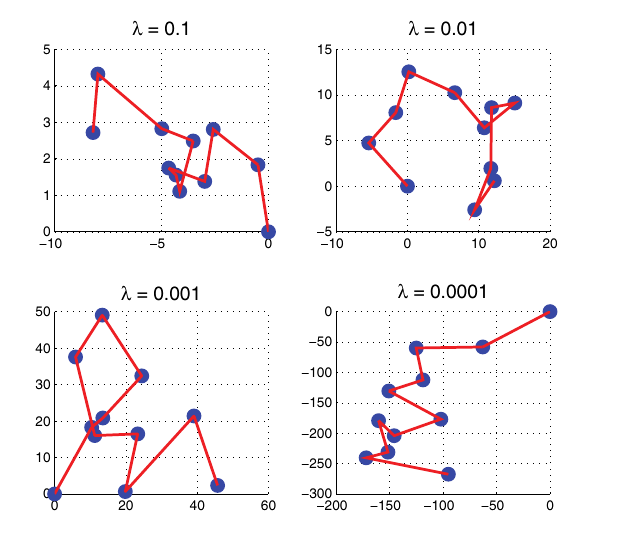
\includegraphics[width=0.6\textwidth]{images/rwpTraces.png}
     \caption[Sample traces of rayleigh RWP mobility model]{\small The transition lengths are statistically shorter with larger mobility parameter $\lambda$, and vice
	versa.\footnotemark}
\end{figure}
\footnotetext{Image Credits: Xingqin Lin et al.}
\end{frame}

\begin{frame}
The mean transition length and time are as follows:
\begin{align*}
	E[L] &= \frac{1}{2\sqrt{\lambda}} \\[2ex]
	E[T] &= \frac{1}{2v\sqrt{\lambda}}
\end{align*}
\end{frame}

\begin{frame}{Sojourn Time} {}
Sojourn time is the amount of time a node resides in the region of interest. Calculating the mean sojourn time is challenging primarily because it involves finding node distribution during each transition. An expression for  mean sojourn time of a cell user during one movement period starting from origin in a hexagonal cell was given in \cite{lin}. We have to note that
a moving node usually makes more than one transition before it leaves
the region. Also, starting from origin implies the node co-exists with BS at
t=0 which is not representative of the distribution of relays/users. Even if we
allow these two assumptions, the problem is still difficult to solve in this
approach as the region has no definite shape like a polygon and finding integration limits is tedious. 
\end{frame}



\begin{frame}{Sojourn Time}{}
	If we know the expected number of transitions $E[N]$ a node makes before moving out of the
region, then sojourn time can be given by
\begin{equation*}
	S_T = (E[N]-1)E[T] + E[T_{last}]
\end{equation*}
where $T_{last}$ is the time spent inside the region during the last transition.
Since it is difficult to characterize $T_{last}$, we approximate $S_T$ to $(E[N]-1)E[T]$. 
\end{frame}



\begin{frame}{E[N]}{}

\begin{equation*}
	E(N) = \sum_{k=1}^{\infty} k Pr(r,\theta,k)
\end{equation*}
where 
\begin{align*}
	Pr(r,\theta,k) &= \int_{S-A} \int_A \ldots \\ &\int_A f_{X_1/X_0}(x_1/x_0)\ldots f_{X_{k+1}/X_{k}}(x_{k+1}/x_{k}) dA_1 \ldots dA_{k+1}
\end{align*} is the probability that the node exits the region during $k+1$ th transition. 
$f_{X_n/X_{n-1}}(x_n/x_{n-1})$ is the probability density of the destination $X_n$ given that
the node's current position is $X_{n-1}$. $X_0 = (r,\theta)$ is where the node starts the  movement at t=0, $A$ is the feasibility region and $S$ is the entire plane. 
\end{frame}






\begin{frame}{Leaving in One Transition}{}
\begin{align*}
	\rho(r,\theta) &= Pr(-\alpha_2 < \alpha < \alpha_1,r_1 > r_{11}) + Pr(\alpha_1 < \alpha < 2\pi-\alpha_2, r_1 > r_{12}) \\
	&= \int_{-\alpha_2}^{\alpha_1} \int_{r_{\!_{11}}}^{\infty} f_{r_1,\alpha}(r_1,\alpha)dr_1 d\alpha +  \int^{2\pi-\alpha_2}_{\alpha_1} \int_{r_{\!_{12}}}^{\infty} f_{r_1,\alpha}(r_1,\alpha)dr_1 d\alpha 
\end{align*}
	This is a general expresion that can be used for any mobility model. In case of RWP,
	$r_1$ and $\alpha$ are chosen independently. Therefore, 
	$f_{r_1,\alpha}(r_1,\alpha) = f_{r_1}(r_1)f_{\alpha}(\alpha)$ 
\begin{align*}
	\rho(r,\theta)&= \int_{-\alpha_2}^{\alpha_1} f_{\alpha}(\alpha) \int_{r_{\!_{11}}}^{\infty} f_{r_1}(r_1)dr_1 d\alpha +  \int^{2\pi-\alpha_2}_{\alpha_1} f_{\alpha}(\alpha) \int_{r_{\!_{12}}}^{\infty} f_{r_1}(r_1)dr_1 d\alpha  \\
	&= \int_{-\alpha_2}^{\alpha_1} \frac{1}{2\pi} e^{-\lambda \pi r_{\!_{11}}^2} d\alpha +  \int^{2\pi-\alpha_2}_{\alpha_1} \frac{1}{2\pi} e^{-\lambda \pi r_{\!_{12}}^2} d\alpha
\end{align*}
\end{frame}



\begin{frame}{Leaving in One Transition} 
The probability with which a 
node at $(r,\theta)$ moves out of the region of interest during the next transition is 
\begin{equation*} 
	\rho(r,\theta) = \int_{-\alpha_2}^{\alpha_1} \frac{1}{2\pi} e^{-\lambda \pi r_{\!_{11}}^2} d\alpha +  \int^{2\pi-\alpha_2}_{\alpha_1} \frac{1}{2\pi} e^{-\lambda \pi r_{\!_{12}}^2} d\alpha
\end{equation*}
%and the sojourn time during this movement is 
%\begin{equation} \label{eq:oneOutProb}
%	S_T = \frac{1}{v}\int_{-\alpha_2}^{\alpha_1} r_{11} \frac{1}{2\pi} e^{-\lambda \pi r_{\!_{11}}^2} d\alpha +  \frac{1}{v}\int^{2\pi-\alpha_2}_{\alpha_1}r_{12} \frac{1}{2\pi} e^{-\lambda \pi r_{\!_{12}}^2} d\alpha \end{equation} \\
Where
\begin{align*}
	r_{\!_{11}} &= -r\cos(\theta -\alpha) + \sqrt{R_0^2 - r^2\sin^2(\theta - \alpha)} \\
	&\\
	r_{\!_{12}} &= R_0 \cos \alpha - r\cos(\theta - \alpha)  \\&+  \sqrt{[R_0 \cos \alpha - r\cos(\theta-\alpha) ]^2 - r^2\sin^2 \theta - [R_0 - r\cos \theta]^2 + R_2^2} \\
\end{align*}
\end{frame}



\begin{frame}{Leaving in One Transition}{}
\begin{align*}
        \beta_2 &= \cos^{-1}\bigg(1-\frac{R_2^2}{2R_0^2}\bigg) 
	\quad
	\beta_1 = \beta_2 - \theta \\
	&\\
	\alpha_1 &= \theta + \tan^{-1}\bigg( \frac{R_0\sin\beta_1}{R_0\cos\beta_1-r}\bigg)\\
			& \\
        \alpha_2 &= \tan^{-1}\bigg( \frac{r\sin\theta + R_0\sin\beta_2}{R_0cos\beta_2 - r\cos\theta} \bigg)
\end{align*}
\end{frame}



\begin{frame}{Simulations} {}

For all simulations, a 1000x1000 square is used to represent the whole 2-D plane. This size is good enough in the sense that using a larger square led to longer runtimes with little to no 
effect on the results. In the mobility model we used, transition length is Rayleigh distributed. To draw a length from Rayleigh distribution, the following method is used:

\begin{enumerate}
	\item Draw a number N from Poisson distribution with density $\lambda A$ where $A$ is the area of the square.
	\item Distribute these N points uniformly on the square 
	\item Of these N points, choose the point that is closest to the point under consideration. 
\end{enumerate}

As discussed in \cite{ganti}, this leads to Rayleigh distribution of transition length and can be proved easily using null probability of a Poisson Point Process. 

\end{frame}


\begin{frame}{Simulations} {}

To test if the above mentioned method introduces any artefacts, let us see how simulated $E[L]$ fares with the formula $E[L] = \frac{1}{2\sqrt{\lambda}}$. Simulated expected length is calculated by averaging transition lengths of 100 traces in each of which the node makes 1000 transitions. 
\begin{figure}[h]
	\centering \vspace{-0.1in}
	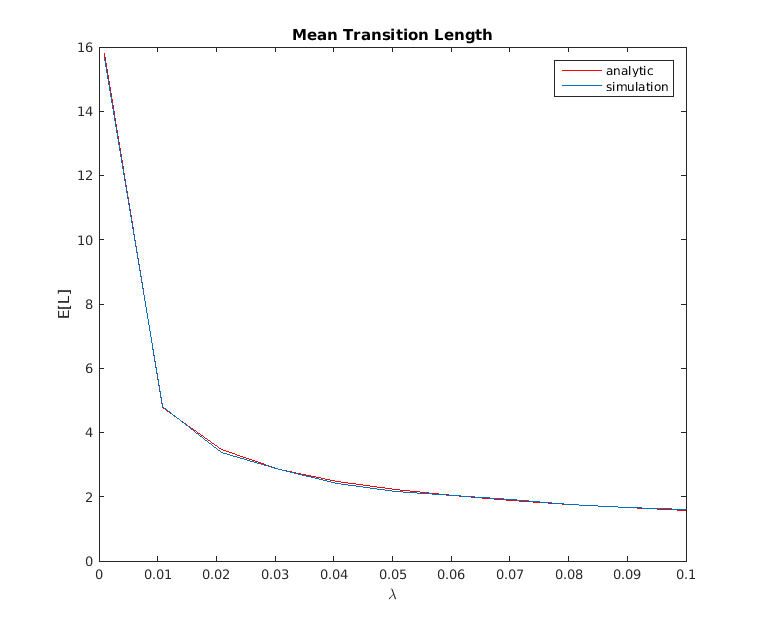
\includegraphics[width=0.75\textwidth]{images/rwpStat.png}
	\vspace{-20pt} \caption[Mean transition length vs. $\lambda$]{Mean transition length vs. $\lambda$}
	\label{fig:rwpEL}
\end{figure}
As seen in the graph \ref{fig:rwpEL}, the simulated value closely follows the analytical formula.

\end{frame}


\begin{frame}{Simulations} {}
 
\begin{figure}[ht!]
    % \begin{center}
%
        \subfigure[\small $\lambda = 0.0005$]{%
            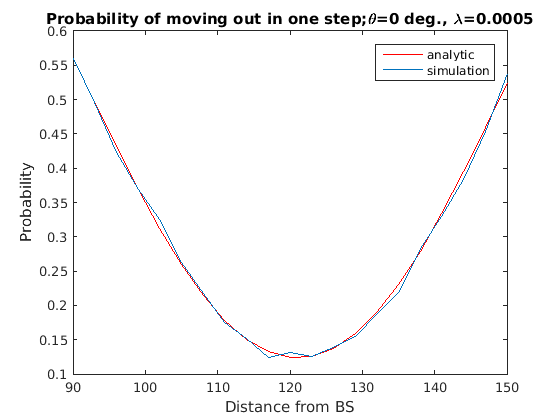
\includegraphics[width=0.55\textwidth]{images/oneOutProbl0005t0.png}
        }%
        %\subfigure[\small $\lambda = 0.001$]{%
        %  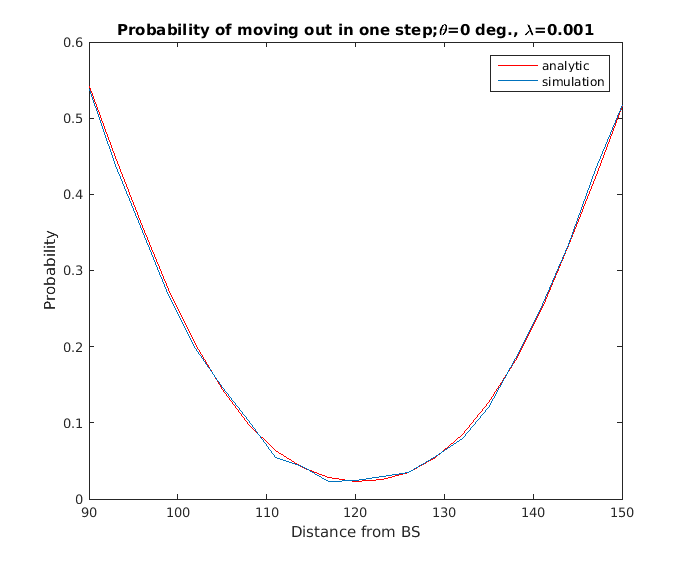
\includegraphics[width=0.42\textwidth]{images/oneOutProbl001t0.png}
        %}\\ %  ------- End of the first row ----------------------%
        \subfigure[\small $\lambda = 0.005$]{%
            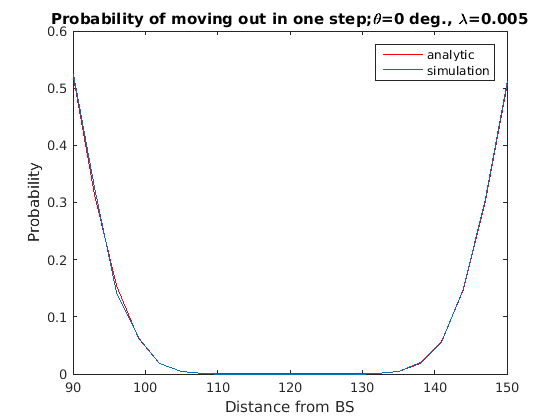
\includegraphics[width=0.55\textwidth]{images/oneOutProbl005t0.png}
        }%

%        \subfigure[Caption of Fourth Figure]{%
%            \label{fig:fourth}
%            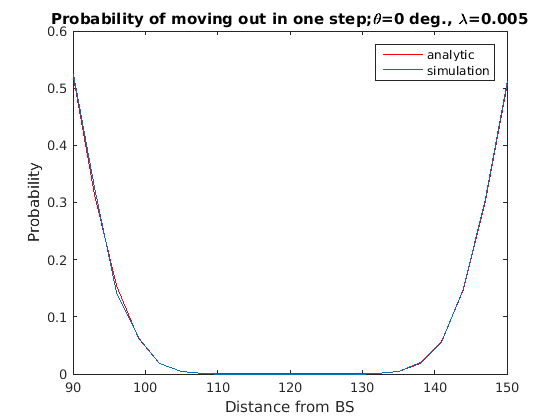
\includegraphics[width=0.4\textwidth]{images/oneOutProbl005t0.png}
        %}%
%
    %\end{center}
	\caption[$\rho(r,0)$ vs. $\lambda$]{\small $\rho(r,0)$ vs. $ \lambda$}%
   \label{fig:vslambda}
\end{figure}

\end{frame}


\begin{frame}{Simulations} {}


\begin{figure}[H]
     \begin{center}
%
        \subfigure[$\theta = 5^{\circ}$]{%
           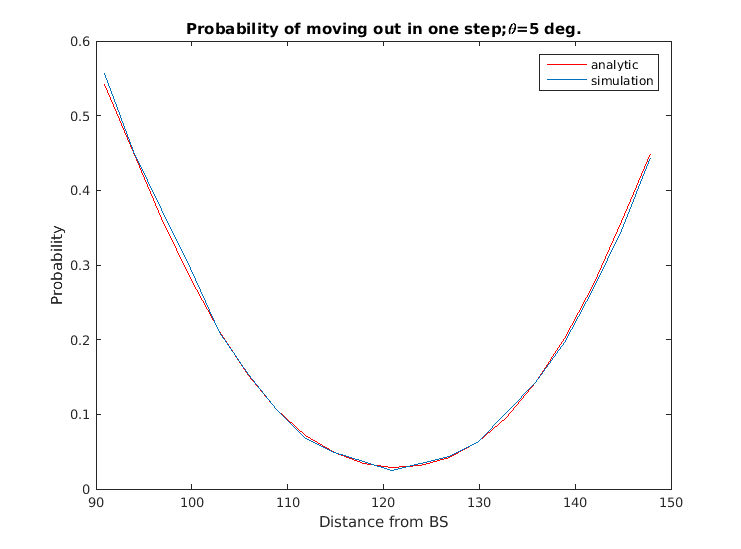
\includegraphics[width=0.42\textwidth]{images/oneOutProb5.png}
        } %  ------- End of the first row ----------------------%
        \subfigure[$\theta = 15^{\circ}$]{%
            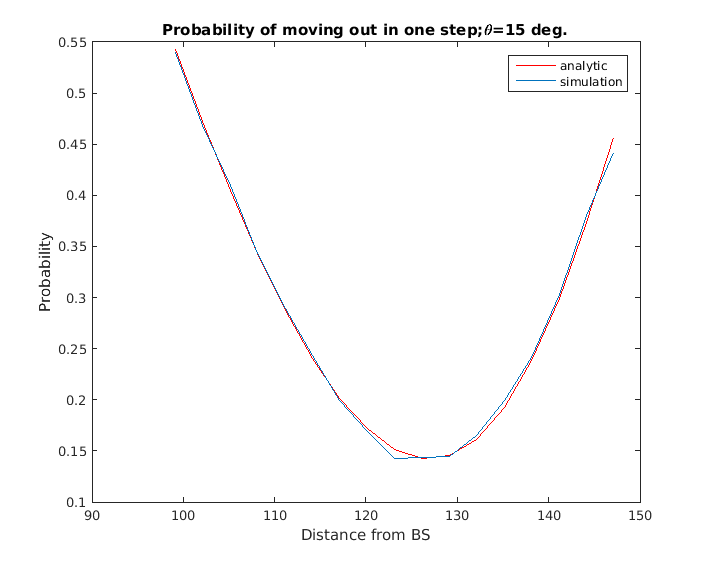
\includegraphics[width=0.42\textwidth]{images/oneOutProb15.png}
        }% \\

        \subfigure[$\theta = 20^{\circ}$]{%
            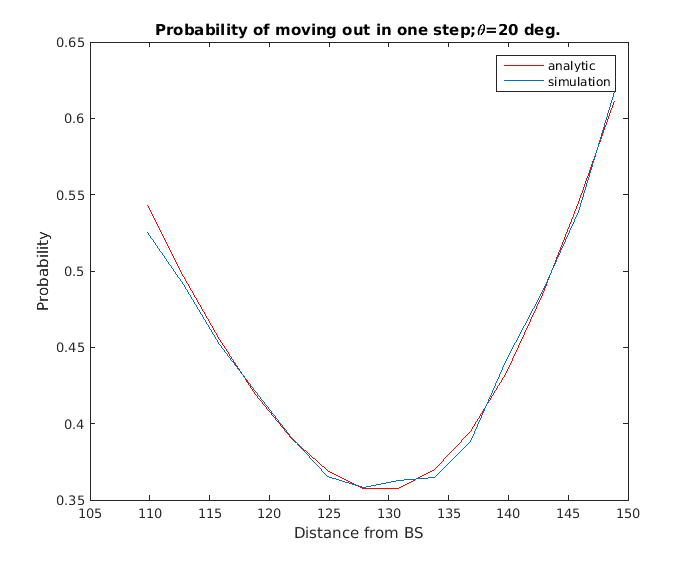
\includegraphics[width=0.45\textwidth]{images/oneOutProb20.png}
        }%
%
    \end{center}
\end{figure}

\end{frame}

\begin{frame}{E[N]}
Let us make a gross approximation and use the same probability of leaving for all waypoints
in the path. Then the average number of steps a node starting at $(r,\theta)$ takes to leave the region is given by
\begin{align*}
	E[N] &= \sum_{k=1}^{\infty} k(1-\rho(r,\theta))^{k-1} \rho(r,\theta) \\[2ex]
	&= \frac{1}{\rho(r,\theta)}
\end{align*}
\end{frame}

\begin{frame}{E[N]}
The plots are for points along the radius at angles $\theta = 10^{\circ}$ and $\theta = 15^{\circ}$. We can see that the analytical formula agrees better for narrower regions. As discussed in Chapter 4, this can be improved by modelling the motion of a node as an absorbing Markov Chain and discretizing the state space.

\begin{figure}[ht!]
     \begin{center}
%
        \subfigure[$\theta = 10^{\circ}$]{%
         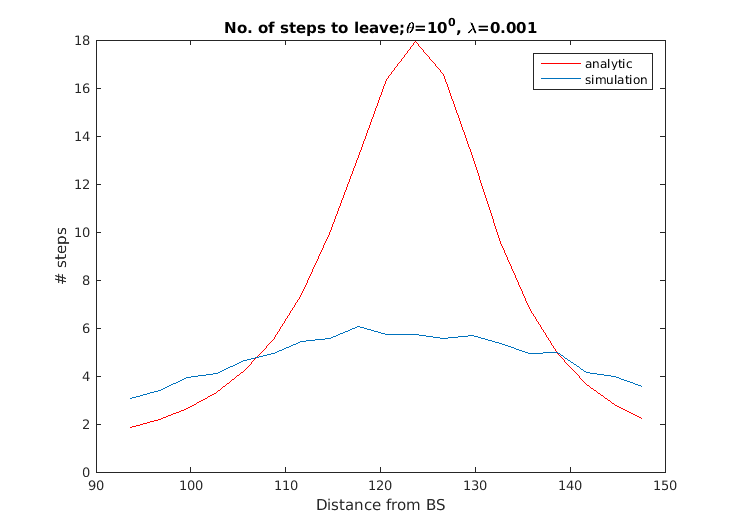
\includegraphics[width=0.42\textwidth]{images/stepst10.png}
        }%
        \subfigure[$\theta = 15^{\circ}$]{%
           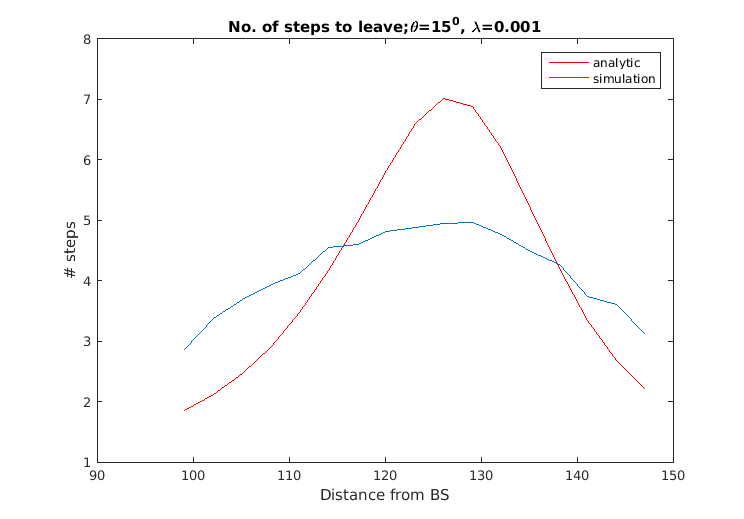
\includegraphics[width=0.42\textwidth]{images/stepst15.png}
        }\\ %  ------- End of the first row ----------------------%
%
    \end{center}
	\caption[Expected number of transitions]{Expected number of transitions}%
   \label{fig:EN}
\end{figure}
\end{frame}


\begin{frame}{Ongoing Work} {Markov Chain Process}
The transitions in this mobility model have Markovian property in the sense that the next waypoint depends entirely on the current position. 
\begin{equation*}
	f_{X_n/X_{n-1},X_{n-2},\ldots,X_0}(x_n/x_{n-1},x_{n-2},\ldots,x_{0}) = f_{X_n/X_{n-1}}(x_n/x_{n-1})
\end{equation*}
Where $X_{n-1}$ is the current waypoint and $X_n$ is the next waypoint. \\
\end{frame}


\begin{frame}{Ongoing Work} {Discretizing State Space}
The idea is to discretize the state space of this Markov chain and model the motion as an 
Absorbing Markov Chain in which the node transitions among the non-absorbing states present 
inside the region before finally moving to the absorbing state. 
Let the whole space be represented by $n+1$ states of which $n$ states lie inside the region 
of interest and the $n+1$th state represents the space outside the region. The transition 
probabilities among first $n$ states depend on the distances between the nodes and the 
transition probabilities from these $n$ states to the absorbing state is $\rho(r_i,\theta_i)$ 
where $(r_i,\theta_i)$ is the position of the $i$th state. We can then use the expressions 
given in \cite{wiki:markovWiki} to find expected value and variance of the number of
transitions a node makes before getting absorbed in the $(n+1)$th state. 
\end{frame}

\begin{frame}
The transition 
probability matrix of this Markov Chain is  
\begin{equation*}
	P  = \left(
	\begin{array}{cc}
	Q & R \\
		\mathbf{0} & 1 \\
	\end{array} \right)
\end{equation*}
	Where $Q_{n \times n}$ is the transition probability matrix of $n$ non-absorbing 
	states and $R_{n\times1}$ contains the probabilities of moving out in one step from 
	each of those $n$ states. 
	 $\mathbf{t}_{n \times 1}$, the vector which contains expected number of transitions, 
	 is given by
\begin{equation*}
	\mathbf{t} = F\mathbf{1}
\end{equation*}
and the variance vector $V$ is given by
\begin{equation*}
	 V = (2F-I)\mathbf{t} - \mathbf{t}_{sq}
\end{equation*}
where $F = \sum_{k=0}^{\infty} Q^k = (I-Q)^{-1}$ is the fundamental matrix.
\end{frame}



\begin{frame}

\begin{itemize}
\frametitle{References} 
\item X. Lin, R. K. Ganti, P. J. Fleming, and J. G. Andrews, “Towards understanding
the fundamentals of mobility in cellular networks,” IEEE Transactions on Wireless
Communications, vol. 12, 2013.

\item S. Shin, U. Lee, F. Dressler and H. Yoon, "Analysis of Cell Sojourn Time in Heterogeneous Networks With Small Cells," IEEE Communications Letters. vol. 20, 2016

\item H. Elkotby and M. Vu, “Interference and throughput analysis of uplink user-assisted
relaying in cellular networks,” PIMRC, 2014.

\item R. K. Ganti, “Stochastic geometry and wireless networks.” SPCOM, July 2012.

\item Wikipedia, “Absorbing Markov Chain - wikipedia, the free encyclopedia,”.

\end{itemize}
\end{frame}


\end{document}
